\chapter{Related Work}
\label{chap:relatedwork}
\numberwithin{equation}{chapter}

This chapter will examine commercial and open-source solutions that provide functionalities similar to Scriburg's. In Section \ref{sec:existing-web-crawlers}, a collection of currently available web crawlers will be presented. In Section \ref{sec:high-level-google-architecture}, we will provide an overview of the architecture of the Google search engine, as some of its fundamental architectural concepts will be adapted with certain modifications.

\section{Existing Web Crawlers}\label{sec:existing-web-crawlers}
The concept of web crawling dates back to the early 1990s when the World Wide Web was still in its infancy.

\textbf{WebCrawler}, created by Brian Pinkerton in 1994 \cite{pinkerton2000webcrawler}, is considered the first actual web crawler-powered search engine. One of the significant innovations of WebCrawler was its \textbf{full-text}\footnote{Full-text search involves electronically searching through extensive text data and retrieving results that contain either some or all of the words from the query.} searchability. This capability made it famous and highly functional. It continues to operate as a search engine, although not as popular as Google, Yahoo, and Bing.

Over the past few decades, web crawlers have evolved significantly, adopting various designs and implementations to crawl and index the internet. They have adapted to address emerging challenges and complexities, such as handling dynamic content, user interactions, authentication, and ethical concerns. Notably, \textbf{Google} is a state-of-the-art search engine dominating the entire market. As of 2023, Google controls a market share of approximately 84\% \cite{statista}, surpassing its closest competitor, Bing, by a significant margin of 75\%. Bing, a well-known search engine developed by Microsoft, has garnered increased attention recently. Nevertheless, given Google's dominance over other search engines, it is reasonable to focus on its solutions and overlook the rest. Furthermore, Google makes some research papers available online, a practice that has yet to be observed among other search engines like Bing, making it easier to study.

Although the previously mentioned search engines offer a wide range of features and are used as generic crawlers to fetch all web pages from the entire internet, they still need to be more general and can not be used and configured to specific personal use cases. Moreover, the most powerful search engines are not free; nobody can clone and modify as they wish. In Section \ref{sec:high-level-google-architecture}, we will understand Google's robust infrastructure, which we will use as a starting point for the Scriburg search engine. However, we must extend it by adding a user interface to make it configurable.

Since using a general search engine like Google directly is currently not an option, data scientists employ various tools to crawl and parse internet content. Each tool has its advantages and disadvantages, depending on distinct use cases. The following list summarizes several widely recognized crawling tools and explains how the proposed solution in this thesis distinguishes itself from them.


\begin{itemize}
  \item[] \textbf{Beautiful Soup:} Beautiful Soup is an open-source library that stands out as a widely used web scraping library that simplifies retrieving data from HTML and XML documents. Beautiful Soup demonstrates exceptional proficiency in parsing HTML documents, streamlining the task of retrieving particular components like headings, paragraphs, tables, and links. Beautiful Soup is not a search engine. It lacks the most fundamental search engine components; hence, it requires programming skills and can only be used to implement a search engine. Beautiful Soup can only parse the first seen page HTML version. Meaning it does not include the JavaScript code. This is bad as most modern web pages use JavaScript heavily to improve the page's latency. For example, \textbf{pagination}\footnote{Website pagination is dividing a long list of content or search results into multiple pages to make it easier for users to navigate and access information.} will be an issue for Beautiful Soup.

  \item[] \textbf{Scrapy:} It is an open-source, powerful, and flexible tool that easily crawls and parses different websites. It allows the creation of custom spiders to crawl multiple pages. Easy to scale makes it suitable for large projects. This tool is perfect for programmers but not for non-technical users, as it requires good knowledge of Python programming. With Scriburg, we aim to reduce the programming workload and save time by offering a user-friendly interface that can be effortlessly configured for individual websites. Moreover, Scrapy also does not render the JavaScript content out of the box and requires an extra library named Splash \footnote{Scrapy documentation: \url{https://docs.scrapy.org/en/latest/topics/dynamic-content.html}}.

  \item[] \textbf{Selenium:} It is an open-source, robust, and adaptable solution for web scraping, automating browser actions, interaction with web pages, and data extraction from online sources. It shares some features with the Beautiful Soup as it is an excellent tool for parsing the HTML DOM. Still, it also overcomes the issue previously mentioned about rendering JavaScript and supporting dynamic contents as pagination. Interactive browser automation makes it easy to mimic the user's behavior, which makes it easier to navigate toward hidden content that requires events and human interactions. Selenium alone can not be used as a search engine; however, it will be used in this thesis as a fundamental tool for the search engine implemented. Its primary role in the implementation will be loading pages and parsing HTML.   

  \item[] \textbf{ParseHub:} Stands out as a web crawler tool with an intuitive User Interface, making it a preferred choice for many data scientists. Its most significant advantage lies in its data extraction simplicity. ParseHub has free and paid plans\footnote{ParseHub plans: \url{https://www.parsehub.com/pricing}}, with the free version allowing users to scrape up to 200 pages per run. While this limitation may prove a bit slow for professional crawling, it suits personal use admirably. However, this tool lacks the ability to fine-tune crawling algorithms and lacks an indexing feature. Given its similarity to the solution implemented in this thesis, it will serve as a valuable point of comparison in the evaluation chapter \ref{chap:evaluation}. 
\end{itemize}

\section{Google High-Level Architecture}\label{sec:high-level-google-architecture}

As highlighted in the prior section, Google's foundational architecture serves as the blueprint for designing Scriburg. Google's search engine architecture provides a comprehensive framework for building a scalable search engine, making it an ideal starting point for any research in this domain. Most code within the Google search engine was developed in C or C++ to ensure efficiency and compatibility with operating systems like Solaris and Linux \cite{brin1998anatomy}. On the contrary, Scriburg is implemented in \textbf{Python 3.10}. This choice was made because, in general, Python has a milder learning curve compared to C and C++, making it more appealing to the majority of data scientists for adjustments and modifications.

Figure \ref{fig:google-arch} shows the basic Google high-level architecture. Google employs a distributed crawler system to retrieve web pages from the internet. The \textit{URL Server} maintains a list of discovered URLs that require crawling, effectively serving as a \textit{load balancer}\footnote{A load balancer is a network device or software application that evenly distributes incoming network traffic across multiple servers or resources to enhance efficiency and ensure high availability.} by dispatching these URLs to available \textit{Crawlers}. The \textit{Crawlers} then download the required documents from the web pages, assign a unique identifier known as a \textit{doc ID} to each page, and store the page content on \textit{Store Servers}. Subsequently, the \textit{Store Servers} compress and archive the pages in a \textit{Repository}.

The next phase involves the \textit{Indexer} component, which decompresses the pages and parses their content. Each document transforms into a set of words referred to as \textit{hits}, where each \textit{hit} records the word and its position within the document. The \textit{Indexer} later organizes these \textit{hits} into \textit{Barrels}. Furthermore, the \textit{Indexer} collects links within the crawled pages and maintains them in an \textit{anchor} file. This \textit{anchor} file contains information about the links and their interrelationships \cite{brin1998anatomy}.


\begin{figure}[h]	
     \centering
     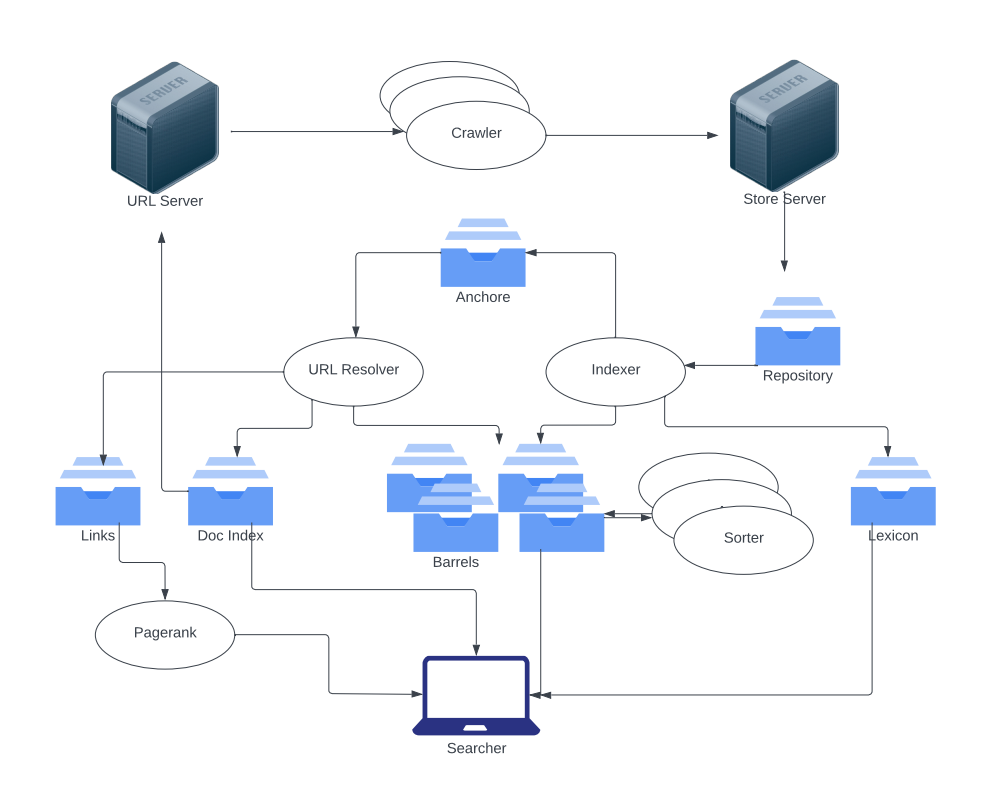
\includegraphics[width=12cm]{figures/google_arch.png}
     \caption{High-level view of Google search engine architecture, showing its main components \cite{brin1998anatomy}.}
     \label{fig:google-arch}
\end{figure}

The \textit{URL Resolver} reads the links from the \textit{anchors'} file and converts the relative URLs into absolute URLs. The URLs are then assigned to their \textit{doc ID}. The links database saves pairs of \textit{doc IDs} that will be used to compute \textit{Page Ranks} for all the documents. 

Initially organized by \textit{doc ID}, the \textit{barrels} are then rearranged by the \textit{sorter} based on \textit{word ID}. This process generates an inverted index. Moreover, the \textit{sorter} generates a list of \textit{word IDs} and corresponding offsets within the inverted index. More explanation about what an \textbf{inverted index} is and how to implement one will be discussed in Section \ref{sec:inverted-index}.
